\section{Background}
Although nobel prize winning Paul Samuelson was widely credited with providing a mathematical basis to Keynesian economics and popularizing the neoclassical synthesis, he was far from the ony economist involved in the movement\autocite{Skousen1997,Samuelson1939}

Another notable Keynesian was Lloyd Metzler who developed a different type of multiplier-accelerator business cycle. Many models developed in the neo-Keynesian era of economics still remain in use but have either been expanded or are used to study specific relationships. Wegener, Westerhoff, and Zaklan expand upon Metzler's inventory cycle model by introducing heterogenous expectations into firm behavior\autocite{Wegener2009}. 

Unlike the well known multiplier-accelerator model developed by Samuelson and Hicks, the dynamics of this model are driven by a Lundberg lag and shifts in the heterogenous mix of behaviors in the firms. The Lundberg lag, named after the eponymous economist Erik Lundberg, is based on a difference existing between the quantity produced and the quantity demanded. This is performed by having firms maintain a level of inventory to absorb unexpected increases in consumption. Firms predict consumption using  one of two behaviors, a regressive type and an extrapolative type. The extrapolative behavior occurs when a firm predicts that future income will deviate from the steady state. The regressive behavior occurs when firms predict that future income will return to the steady state. 

\section{Model Set-Up}
In this business cycle model, the economy is closed and income is determined completely by the quantity of goods produced by firms. Goods are completely homogenized but can be produced for 3 purposes: stock $S$, consumption $U$, and investment $I$. This lets us define income as:
\begin{equation}
    Y_t=I_t+S_t+U_t
\end{equation}
Investment is held to be exogenously determined and constant, thus:
\begin{equation}
    I_t=\bar I
\end{equation}
Consumption adapts to income according to the marginal propensity to consume, $b$. As this model follows closely to the framework developed by Metzler\autocite{Metzler1941}, consumption adapts directly to the current income level as follows:
\begin{equation}
    C_t=bY_t
\end{equation}
Producers have a desired level of inventory based on the expected level of consumption goods. Thus setting, $k>0$:
\begin{equation}
    \hat Q_t=kU_t
\end{equation}  
where $Q$ is the level of inventory. In order to achieve this desired level of inventory, firms produce $S$ amount of output such that:
\begin{equation}
    S_t=\hat Q_t-Q_{t-1}
\end{equation}
However, the expected level of consumption does not necessarily match the produced level of goods. The realized level of inventory change can thus be determined as:
\begin{equation}
    Q_t=\hat Q_t-(C_t-U_t)
\end{equation}

The quantity of goods produced for consumption is determined by firms expectations for desired consumption. The extrapolative expectation rule is used by firms that believe consumption levels will continue shifting away from the long-run average quantity. This behavior is interpreted mathematically as:
\begin{equation}
    U^E_t=C_{t-1}+c(C_{t-1}-\bar C)
\end{equation}
where $c\geq 0$ denotes the speed at which firms expect consumption to deviate from the long-run level. 

The other possible strategy firms can take is to expect consumption to return to the equilibrium level. This is described as the regressive expectation rule and is interpreted mathematically as:
\begin{equation}
    U_t^R=C_{t-1}+f(\bar C-C_{t-1})
\end{equation}
where $0\leq f\leq 1$ denotes the expected adjustment speed to the long-run level. 

As this economy only involves two expectation rules, the aggregate expected level of consumption is a simple weighted average:
\begin{equation}
    U_t=w_tU_t^E+(1-w_t)U_t^R
\end{equation}
The weight is defined as a function of consumption level which allows firms to switch their predictive behavior based on the current consumption level. Intuitively, as consumption deviates further from equilibrium, more firms will believe that the boom or slump will end and adjust in accordance. Likewise, when consumption is close to equilibrium, firms will believe it to be more accurate to extrapolate consumption. This behavior is modelled by the function:
\begin{equation}
    w_t=\frac{1}{1+d(\bar C-C_{t-1})^2}
\end{equation}
where $d$ is proportional to the popularity of the regressive rule.

Taking these rules in aggregate, income is a second-order nonlinear iterated mapping. Condensing the model, we arrive at the mapping:
\begin{equation}
    Y_t=U_t+kU_t-(1+k)U_{t-1}+C_{t-1}+\bar I
\end{equation}
This gives a single fixed point of:
\begin{equation}
    \bar Y=\frac{1}{1-b}\bar I
\end{equation}

It is apparent that, as $\bar Y$ is constant, the theoretical set-up of the model is only valid if there is no long-term growth, that is to say income must be bounded. This is because the predictive mechanism used by firms is reliant on the difference between the lag in consumption and the steady-state level of consumption. If consumption were to consistently grow, then this difference would also grow over time, eliminating any effective purpose in providing heterogenous expectations as firms would practically unanimously switch to the extrapolative mechanism. 

\begin{figure}
    \centering
    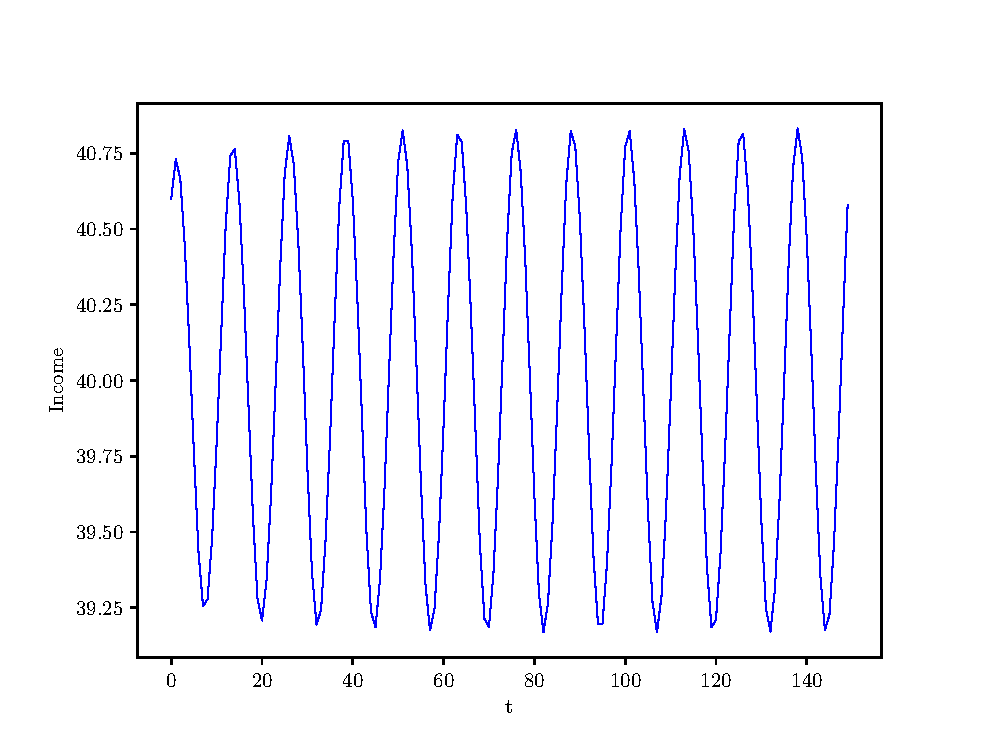
\includegraphics[height=0.4\textheight]{./metzlerian_basic/timeseries_income.eps}
    \caption{Timeseries plot of inventory cycle as described by Wegener et al.\autocite{Wegener2009} Simulation is determined given $Y_0=40.6$, $U_0=30.3$, and $\bar I=10$. The parameters of the model are: $b=0.75,c=0.3,d=1.0,f=0.1,k=0.1$.}
    \label{metzler_basic_timeseries}
\end{figure}

\section{Analysis of Income Dynamics}
In the example trajectory given above, income clearly followed bounded, cyclic behavior. As seen with the analysis of the logistic map however, there are other types of long-term behavior possible. Given the restrictions on parameters, the steady-state level of income is stable if:
\begin{equation}
    k<\frac{1-b-bc}{b(1+c)}
\end{equation}
The proof for this can be seen in the appendix of Wegener et al.\autocite{Wegener2009} The stability of the steady state is only dependent on $b$, $k$, and $c$, thus the behavior of the regressive expectation rule and the ratio of firms behaving with each expectation rule do not affect the stability of this fixed point. This can be seen graphically using bifurcation diagrams of the parameters.

\begin{figure}
    \centering
    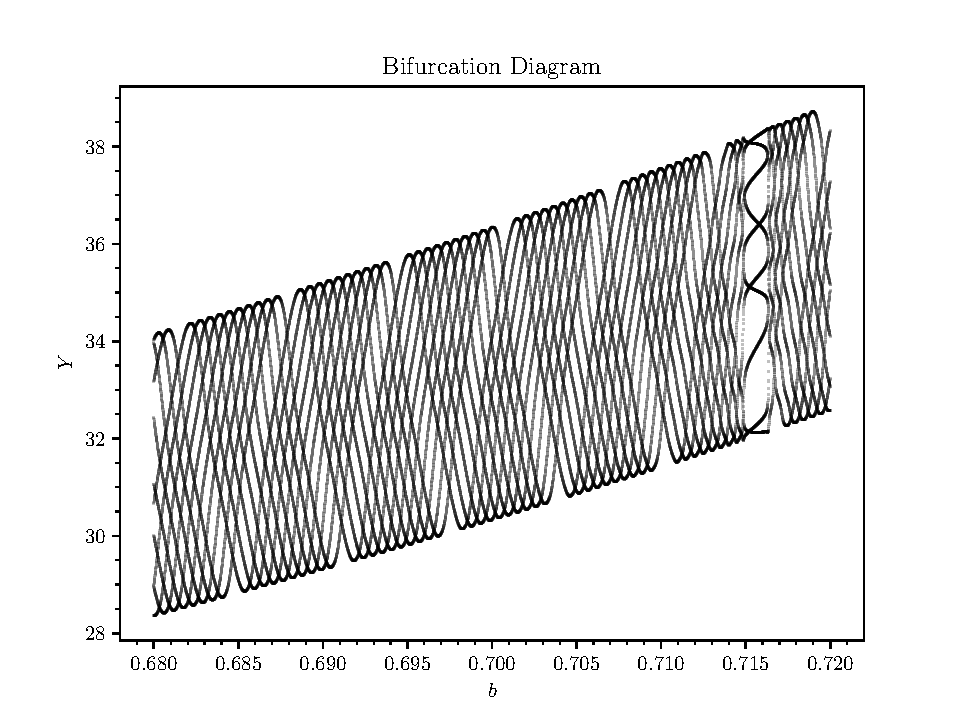
\includegraphics[height=0.4\textheight]{./metzlerian_basic/bbifurcation.eps}
    \caption{Bifurcations diagram varying the parameter $b$ over the range [0.2, 0.85] holding all other parameters and initial conditions as described in Figure \ref{metzler_basic_timeseries}. The simulation was allowed to run for 1000 iterations and the last 50 points are captured in the diagram.}
    \label{metzler_basic_bbifurcation}
\end{figure} 

\begin{figure}
    \centering
    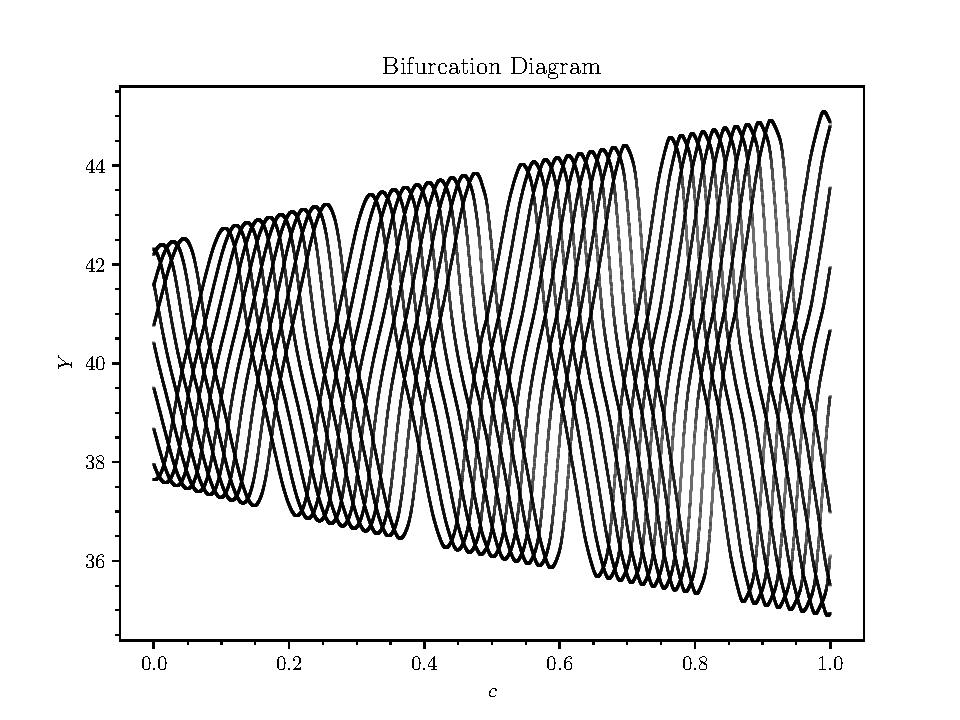
\includegraphics[height=0.4\textheight]{./metzlerian_basic/cbifurcation.eps}
    \caption{Bifurcations diagram varying the parameter $c$ over the range [0.1, 0.9] holding all other parameters and initial conditions as described in Figure \ref{metzler_basic_timeseries}. The simulation was allowed to run for 1000 iterations and the last 50 points are captured in the diagram.}
    \label{metzler_basic_cbifurcation}
\end{figure} 

\begin{figure}
    \centering
    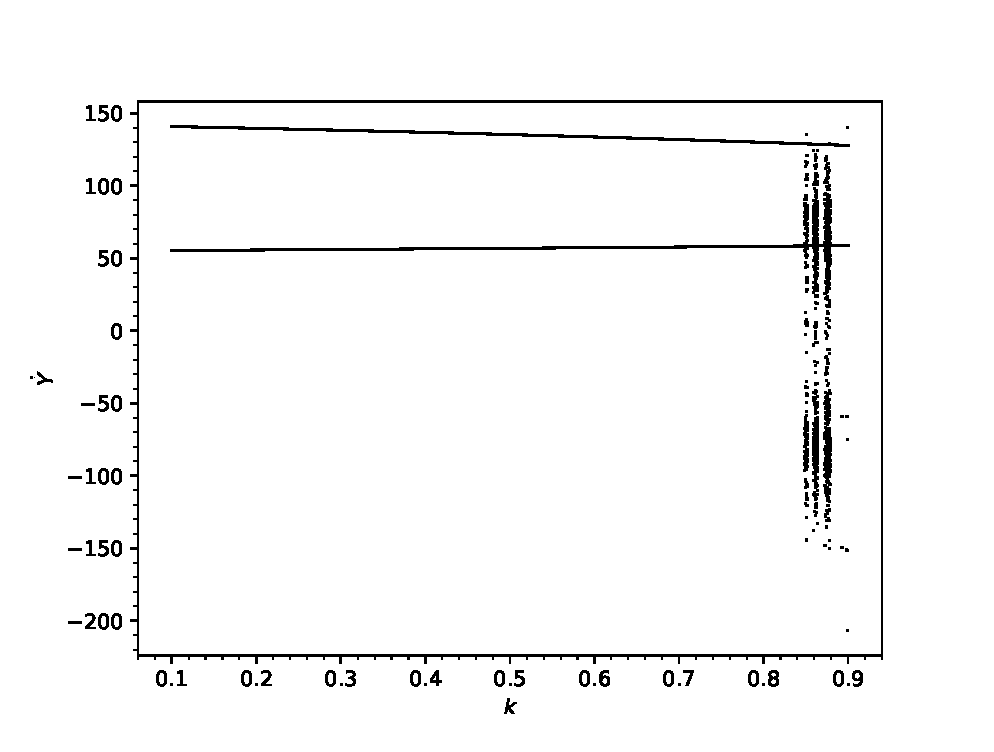
\includegraphics[height=0.4\textheight]{./metzlerian_basic/kbifurcation.eps}
    \caption{Bifurcations diagram varying the parameter $k$ over the range [0.1, 0.4] holding all other parameters and initial conditions as described in Figure \ref{metzler_basic_timeseries}. The simulation was allowed to run for 1000 iterations and the last 50 points are captured in the diagram.}
    \label{metzler_basic_kbifurcation}
\end{figure} 

There is a Neimark-Sacker bifurcation where $b\approx0.65$ which marks a transition point from a stable fixed point to a bounded cycle. However, as $b$ approaches 1, the bifurcation diagram does not graphically feature cycles of well defined order. Varying $c$ and $k$ alters the behavior of the cycles as seen in Figure \ref{metzler_basic_cbifurcation} and \ref{metzler_basic_kbifurcation}. Altering $d$ or $f$ affects the magnitude of the inventory cycles but does not have any effect on the presence of the cycles.

\begin{figure}
    \centering
    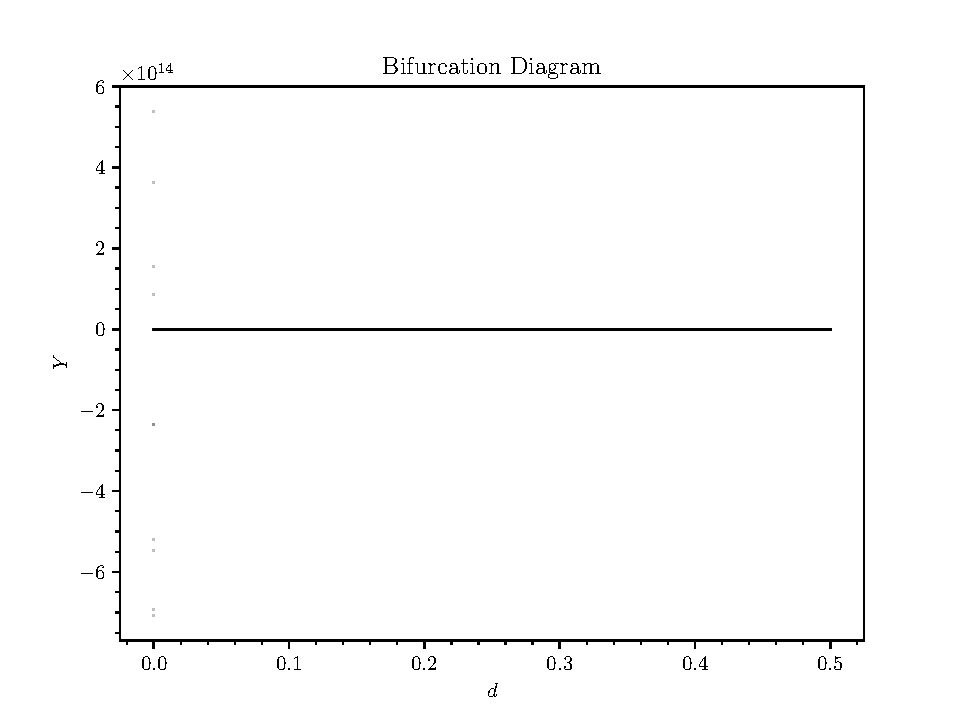
\includegraphics[height=0.4\textheight]{./metzlerian_basic/dbifurcation.eps}
    \caption{Bifurcations diagram varying the parameter $d$ over the range [0.01, 2.0] holding all other parameters and initial conditions as described in Figure \ref{metzler_basic_timeseries}. The simulation was allowed to run for 1000 iterations and the last 50 points are captured in the diagram.}
    \label{metzler_basic_dbifurcation}
\end{figure} 

\begin{figure}
    \centering
    
\includegraphics[height=0.4\textheight]{./metzlerian_basic/fbifurcation.eps}
    \caption{Bifurcations diagram varying the parameter $f$ over the range [0.1, 0.5] holding all other parameters and initial conditions as described in Figure \ref{metzler_basic_timeseries}. The simulation was allowed to run for 1000 iterations and the last 50 points are captured in the diagram.}
    \label{metzler_basic_fbifurcation}
\end{figure}

The bifurcation diagrams varying the $c,\ k,\ d,$ and $f$ parameters appear to display clear cyclic behavior. However, this is actually a product of the graphical display of the bifurcation diagram. The diagram is constructed by iterating the mapping over 1000 time periods and displaying the results of the last 50 time-periods. This results in the appearance of 50-cycles over the span of the bifurcation diagram; however, reducing or increasing the amount of iterations to display likewise changes the apparent periodicity of the cycle. This implies the presence of more points in the long-run trajectories than is visible in the diagram.

